\documentclass[12pt]{standalone}
\usepackage{tikz}
\usetikzlibrary{arrows.meta, positioning, shapes}

\begin{document}

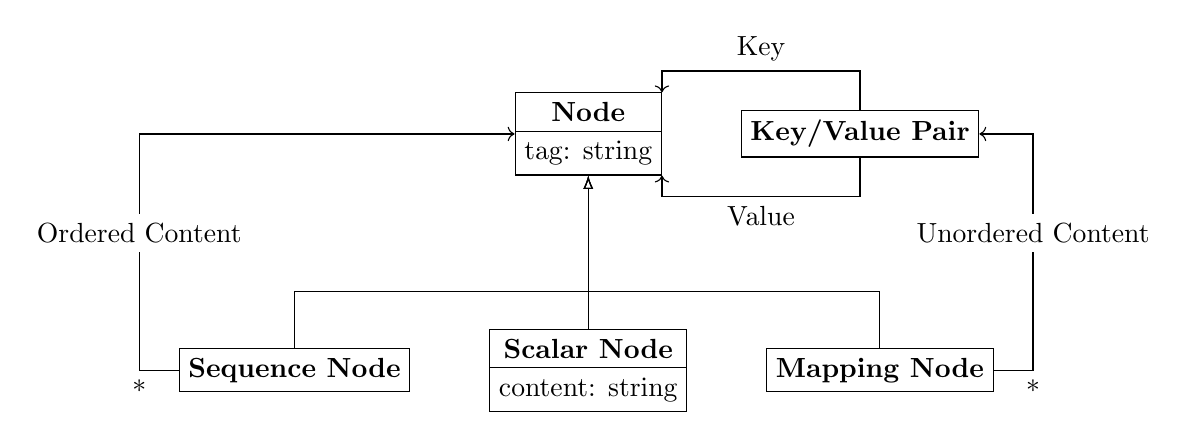
\begin{tikzpicture}[
    entity/.style = {draw=black, rectangle, anchor=north},
    entityAttrs/.style = {draw=black, rectangle split, rectangle split parts=2, anchor=north},
    onArrow/.style = {fill=white, text centered},
    inherits/.style = {-{Latex[open]}},
    node distance=3cm and 1cm,
    auto
]
\node(Node)[entityAttrs] {
    \textbf {Node}
    \nodepart{second} tag: string
};

\node(Scalar)[entityAttrs, below of=Node] {
    \textbf {Scalar Node}
    \nodepart{second} content: string
};
\draw[inherits] (Scalar) -- (Node);

\node(Sequence)[entity, left=of Scalar] {
    \textbf {Sequence Node}
};
\draw[inherits] (Sequence) -- ++(0,+10mm) -| (Node);

\draw[->] (Sequence.west) -| ++(-5mm, 0) |- (Node)
    node[at start, below] {*}
    node[pos=0.25, above, fill=white] {Ordered \linebreak Content};

\node(Mapping)[entity, right=of Scalar] {
    \textbf {Mapping Node}
};
\draw[inherits] (Mapping) -- ++(0,+10mm) -| (Node);

\node(KeyValue)[entity, right=of Node] {
    \textbf {Key/Value Pair}
};

\draw[->] (Mapping.east) -| ++(+5mm, 0) |- (KeyValue)
    node[at start, below] {*}
    node[onArrow, pos=0.25, above] {Unordered \linebreak Content}
    ;

\draw[->] (KeyValue.north)
    -- ++(0,+5mm)
    -| (Node.north east)
    node[pos=0.25, above] {Key}
;

\draw[->] (KeyValue.south) -- ++(0,-5mm) -| (Node.south east)
    node[pos=0.25, below] {Value};

\end{tikzpicture}

\end{document}
